% This is a basic Math Paper

\documentclass[11pt]{article}

% Preamble

\usepackage[margin=1in]{geometry}
\usepackage{amsfonts, amsmath, amssymb}
\usepackage{fancyhdr, float, graphicx}
\usepackage[utf8]{inputenc} % Required for inputting international characters
\usepackage[T1]{fontenc} % Output font encoding for international characters
\usepackage{fouriernc} % Use the New Century Schoolbook font
\usepackage[nottoc, notlot, notlof]{tocbibind}
\usepackage{url}
\usepackage{placeins}
\usepackage{multirow}
% Header and Footer
\pagestyle{fancy}
\fancyhead{}
\fancyfoot{}
\fancyhead[L]{\textit{\Large{Experiment 2: Diffraction Grating}}}
%\fancyhead[R]{\textit{something}}
\fancyfoot[C]{\thepage}
\renewcommand{\footrulewidth}{1pt}



% Other Doc Editing
% \parindent 0ex
%\renewcommand{\baselinestretch}{1.5}

\begin{document}
	
	\begin{titlepage} 
		\centering 
		
		%---------------------------NAMES-------------------------------
		
		\huge\textsc{
			MIT World Peace University
		}\\
	
		\vspace{0.75\baselineskip} % space after Uni Name
		
		\LARGE{
			Physics\\
			First Year B. Tech, Trimester 3\\
			Academic Year 2021-22
		}
		
		\vfill % space after Sub Name
		
		%--------------------------TITLE-------------------------------
		
		\rule{\textwidth}{1.6pt}\vspace*{-\baselineskip}\vspace*{2pt}
		\rule{\textwidth}{0.6pt}
		\vspace{0.75\baselineskip} % Whitespace above the title
		
		
		
		\huge{\textsc{
				Diffraction Grating
			}} \\
		
		
		
		\vspace{0.5\baselineskip} % Whitespace below the title
		\rule{\textwidth}{0.6pt}\vspace*{-\baselineskip}\vspace*{2.8pt}
		\rule{\textwidth}{1.6pt}
		
		\vspace{1\baselineskip} % Whitespace after the title block

		%--------------------------SUBTITLE --------------------------	
			
		\LARGE\textsc{
			Experiment No. 2
		} % Subtitle or further description
		\vfill
		
		%--------------------------AUTHOR-------------------------------
		
		Prepared By
		\vspace{0.5\baselineskip} % Whitespace before the editors
		
		\Large{
			109054. Krishnaraj Thadesar
			
			Division 9 Batch I3
		}
		
		
		\vspace{0.5\baselineskip} % Whitespace below the editor list
		\today

	\end{titlepage}

	\begin{center}
	{\Large Pledge}\\
	\vspace{0.5cm}
	I solemnly affirm that I am presenting this journal based on my own experimental work. I have neither copied the observations, calculations, graphs and results from others nor given it to others for copying.\\
		\end{center}
	
	\vspace{0.5cm}
	
    \begin{flushright}
	{\large Signature of the student}\\
	\vspace{1cm}
	 \end{flushright}
	
	
	
	\begin{center}
		{\LARGE Experiment 2: Diffraction Grating}\\
	\end{center}

	\section{Aim}
	\noindent
To measure the wavelengths of spectral lines of a Mercury (Hg) source using diffraction
grating and a spectrometer.
	
	\section{Apparatus}


		\begin{enumerate}
			\item Diffraction grating
			\item Spectrometer
			\item Mercury source (Hg)
			\item Spirit level
			\item Reading lamp and reading lens
		\end{enumerate}


	\section{Significance of the Experiment}
	\textit{Diffraction grating is basically a super-prism. It disperses the light in to its spectrum, with dispersive power and resolving power quite higher than that of
		prism. The grating assists an analytical technique called spectroscopy in the formation and
		analysis of spectra.}
	
	
	\section{Theory}
 Diffraction grating is an arrangement of large number of equidistant and parallel slits
(Fig 2.1). One of the techniques to manufacture diffraction grating is to rule the equidistant lines
on glass plate. Typical diffraction gratings consist of 15000-20000 lines per inch (this number
can reach up to 100000 lines per inch). The qualities i.e. dispersive power and resolving power
depend upon number of slits and slit density.
Using theory of diffraction to multiple slits, following grating equation can be derived\\
\clearpage
	$$
	d \sin \theta=m \lambda
	$$
	Where
	$$
	\begin{aligned}
		&d=\text { grating element } \\
		&\theta=\text { angle of diffraction } \\
		&m=\text { order of spectrum } \\
		&\lambda=\text { wavelength of light }
	\end{aligned}
	$$
	\begin{figure}[H]
		\centering
		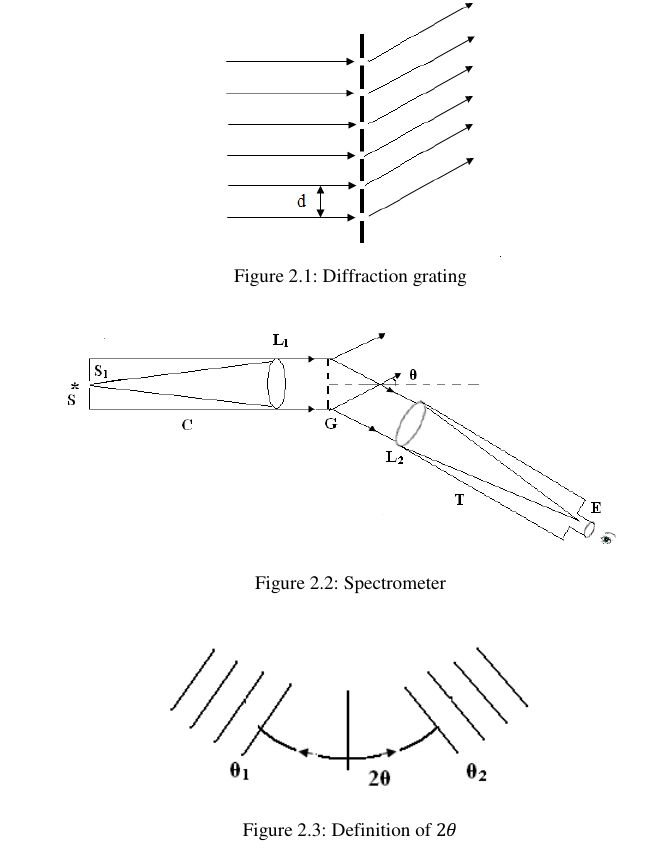
\includegraphics[scale=0.7]{theory.png}
		\label{it}
	\end{figure}
	
	In equation (2.1), d and m are constant. This implies that $\theta$ is proportional to $\lambda$. Thus if a grating
	is exposed to light from polychromatic source, the colors are separated on account of their
	different wavelengths. Thus diffraction grating can form the spectrum of the light. With respect
	to dispersive power and resolving power, grating is far better than prism. Further, if d and m are
	known and if $\theta$ is measured then $\lambda$, the wavelength of spectral lines can be calculated. Due to its
	ability to form well resolved spectrum and calculation of wavelengths, diffraction grating finds
	applications in spectrometers. Such spectrometers (Fig 2.2) find applications in an important
	discipline called spectroscopy, a technique extremely useful in science and technology. Each
	source has its own characteristic spectrum. In spectroscopy the spectra of various atomic or
	molecular species are analyzed to evaluate the properties of the sources. A few applications of
	spectroscopy are - understanding the structure and properties of atoms and molecules, detection
	of various elements in planets and stars, study of various effects such as Zeeman effect, Raman
	effect, Stark effect etc.
	
	\section{Procedure}
	
	\begin{enumerate}
		\item 	1. At first calculate the grating element $d$ of the grating by using following formula
		$$
		d=\frac{1}{N} \text { inches }=\frac{2.54}{N} \mathrm{cms}=\frac{2.54 \times 10^{8}}{N} A^{o}
		$$
		Where $\mathrm{N}=$ Number of slits per inch $=15000$ slits per inch
	
		\item Switch on the Mercury source.
	
	\item Level the all parts of spectrometer such as telescope, collimator, grating table etc. using spirit level.
	\item Bring the slit of collimator in front of spectrometer. Adjust the slit width optimum value.
	\item Adjust the telescope and collimator for sharp images using prism and Schuster's method
	\item Mount the diffraction grating on the table such that it's plane is exactly perpendicular to collimator axis as well as the table
	\item Observe the central image of slit through telescope. This image is white, as colors cannot be separated in zero ${ }^{\text {th }}$ order. This is called as zero ${ }^{\text {th }}$ order spectrum. Make the image sharp by focusing the telescope and collimator
	\item Unlike prism, grating produces multiple spectra. Move the telescope on both sides of the central image to observe the first as well as second order spectra on both the sides of the central image. The second order spectrum is faint as compared to first order. So consider first order spectrum for observations. Thus the order of spectrum $m$ in Eqn (2.1) is 1. The first order spectrum consists of four prominent lines namely violet, green, yellow (doublet) and red. The other relatively faint lines are purple and orange.
	\item Move the telescope on left hand side and adjust the cross wire on violet line. Clamp the telescope. Measure the angular position $\theta_{1}$ of the violet line, by using following procedure
$$
\theta_{1}=M S R+V S R \times L C
$$
Where MSR: Main scale reading: a reading on the scale which coincides with the zero of the vernier scale. If no reading coincides then MSR is the reading on the main scale previous to zero of the vernier scale.
VSR: Vernier scale reading is the sequence number of the division on the vernier scale which exactly coincides with the division on main scale $\mathbf{L C}=$ Least count of the angular scale.



$$
L C=\frac{\text { Smallestdivisiononthemainscale }(X)}{\text { Numberofdivisionsonthevernierscale }(Y)}=\frac{o}{=}=\cdots . \text { minute }
$$
	\item Now unclamp the telescope and move it on right side of the central image and focus the cross wire on the violet line. Measure its position $\theta_{2}$ by using the procedure in step 9 .
	\item Calculate $\theta$ by using following procedure
$$
2 \theta=\left|\theta_{2}-\theta_{1}\right| \text { and } \theta=\frac{2 \theta}{2}
$$
	\item Calculate the wavelength of violet line by substituting $\theta$ in the following Eqn.
$$
\lambda_{e}=\frac{d \sin \theta}{m}
$$
Where $d=$ grating element as calculated in step 1 $m=$ order of the spectrum $=1$
	\item Calculate the percentage deviation by using following formula
$$
\% \text { deviation }=\left|\frac{\lambda_{e}-\lambda_{s}}{\lambda_{s}}\right| \times 100 \%
$$
Where $\quad \lambda_{e}=$ experimental wavelength as calculated in step (12) $\lambda_{s}=$ standard wavelength, given in the table $2.1$
	\item Repeat the same procedure in step 9 to 13 for remaining spectral lines i.e. green, yellow and red.
	\item Tabulate your observations, calculations and results in table 2.1.


	\end{enumerate}
\clearpage

	\section{Observations}

Table (2.1) Observations, Calculations and Results
$$
\begin{aligned}
	&d=\text { grating element }=d=\frac{2.54 \times 10^{8}}{N} A^{o}=\frac{2.54 \times 10^{8}}{15000} A^{o}= \\
	&m=\text { order of the spectrum }=1
\end{aligned}
$$

	\begin{figure}[H]
	\centering
	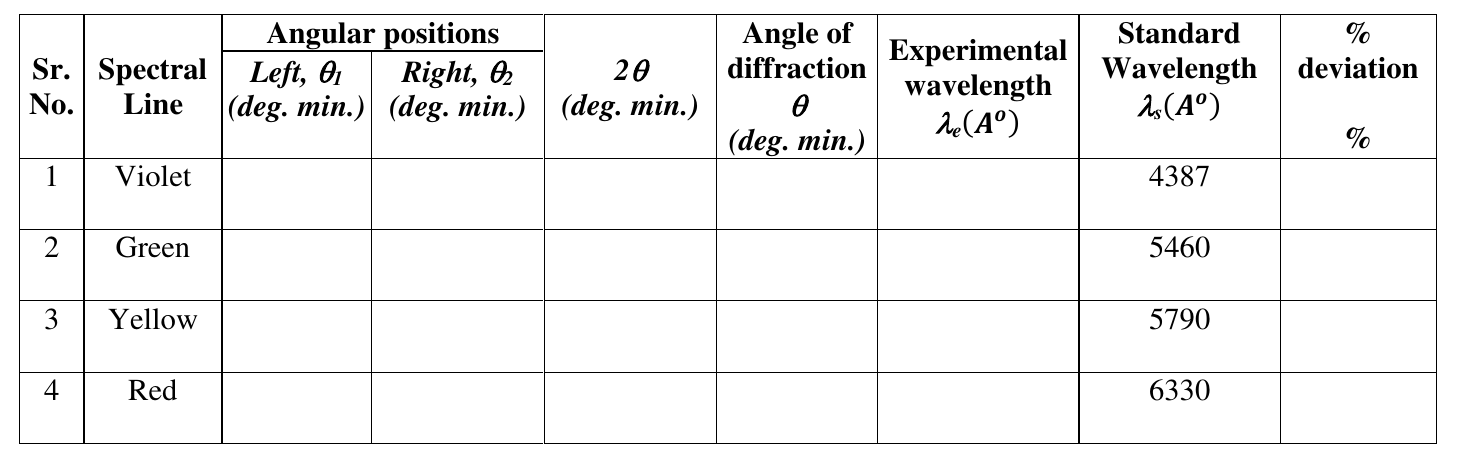
\includegraphics[scale=0.45]{table.png}
	\label{it}
\end{figure}

	\section{My Understanding of the Experiment}
	Diffraction is when light waves bend around an object. In a diffraction grating, the rays of light have thousands of slits in front of them, and therefore each wave diffracts with its respective slit, causing it naturally interfere with the other waves near it. This makes us see the individual wavelengths of light on the screen.  
	
	Because of this, we can essentially clearly split polychromatic light into its monochromatic sources, and this has a vast array of applications. \textit{From looking at stars, and matching their emmision spectra with known elements to determing their age, to just splitting mercury light into its individual frequencies. }

\end{document}